%This work is licensed under the Creative Commons Attribution-NonCommercial-NoDerivs 3.0 United States License. To view a copy of this license, visit http://creativecommons.org/licenses/by-nc-nd/3.0/us/ or send a letter to Creative Commons, 444 Castro Street, Suite 900, Mountain View, California, 94041, USA.

\section{Accelerator Design} \label{sec:gun_design}

The acceleration region of our prototype UEM system has several requirement which are unique in comparison to standard electron guns.
As discussed in \ref{chap:considerations} notable requirements include the need to handle a large photoemission area and the inability to employ a pin-hole to selectively clean the electron beam.
This concern leads to several additional criteria.
The system must first be able to accept the large laser spot size needed to generate the electron beam.
Then, in order to accomodate this large electron pulse, both the cathode Wehnelt and anode aperture must be similarly large; in fact, the beam size at the anode aperture will typically be larger than at the emission source due to beam expansion during acceleration.
Also, care must be taken to ensure a relatively uniform electric field for acceleration of the pulse.
While in transit from the cathode to the anode, this large beam is more susceptable to non-uniformities in the electic field given that it will span a wider proportion of the accelerator than the thin beams used in conventional TEM.

\begin{figure}
  \centering
  \centerline{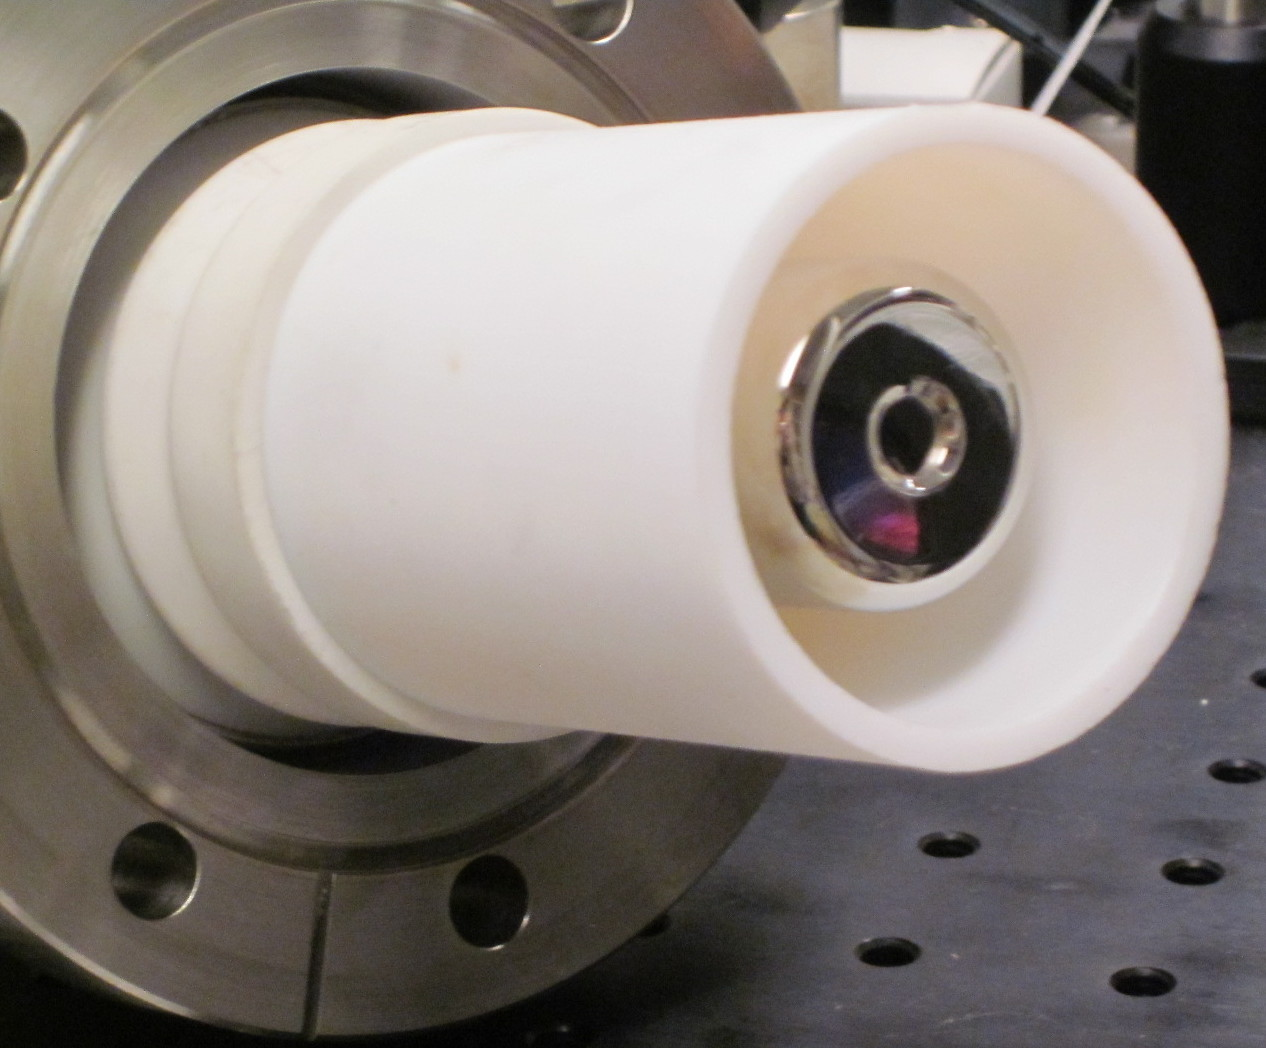
\includegraphics{cathode.jpg} 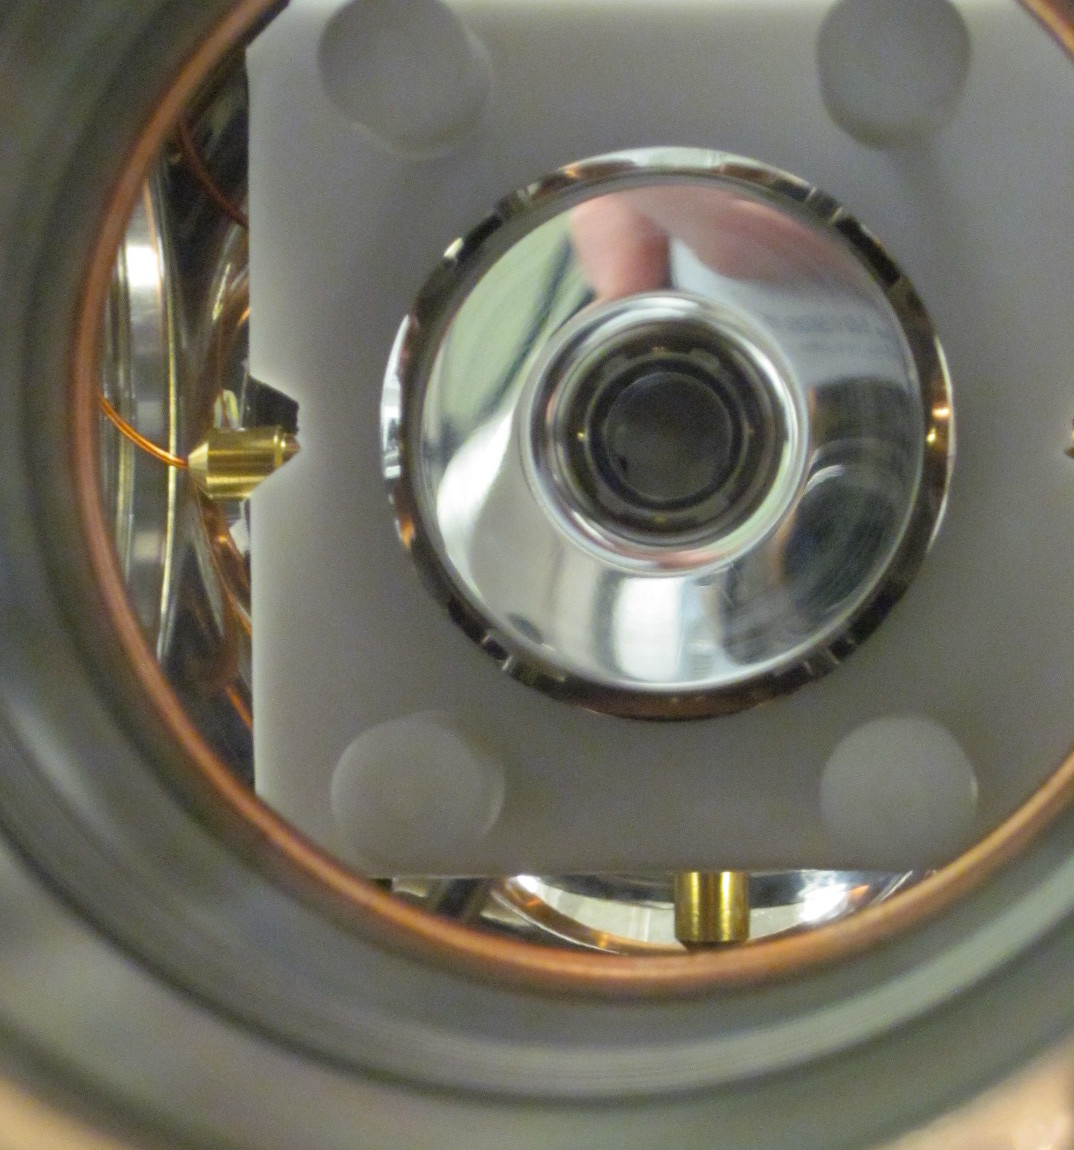
\includegraphics{anode.jpg}}
  \caption[Pictures of the employed Togawa-inspired custom cathode-anode pair]{
    Pictured are the cathode (left) and anode (right) of the accelerator built at UIC from a design by Togawa \protect\textit{et al.} \protect\cite{togawa_ceb6_2007}.
    The photocathode is visible in the cathode Wehnelt aperture.
    The anode is viewed as installed in the column, through the opened port normally occupied by the cathode and high voltage feedthrough.
    The white material seen in both images helps to prevent electrical arcing under high voltage.
  }
  \label{fig:togawa-pic}
\end{figure}

These requirements lead to the fabrication of cathode/Wehnelt and anode pair based on the design of Togawa \textit{et al.} \cite{togawa_ceb6_2007} (pictured in \ref{fig:togawa-pic}).
A schematic of this design, overlayed by a Finite Element Model (FEM) simulation of the electic field, is shown in \ref{fig:gun-field}.
The simulation was performed using \texttt{FreeFEM++}, a free finite element partial differential equation solver and meshing toolkit (\url{http://www.freefem.org/ff++/index.htm}).
The FEM simulation modeled the features of the anode and cathode, while emulating gap walls at infinity by placing a linear potential on gap edges at a large distance.
From the field equipotentials, it is clear that this design has a consistently flat electric field for large displacements off the central axis.
Since the shape of the field is scale independent, the schematic shows that the aperture width and laser acceptance concerns are easily satisfied for an appropriate choice of scale.

\begin{figure}
  \centering
  \begin{tikzpicture}
  \node at (0,0) {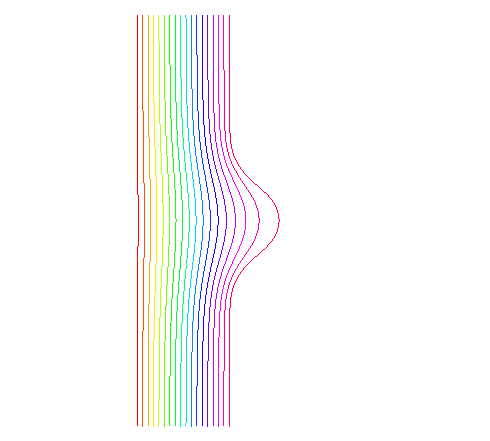
\includegraphics{gunfield.png}};
  \draw [fill=blue!40]
    (-1.4,-3.1)
    -- ++(0,6.2)
    -- ++(-1.1,0)
      node [above, pos=0.5] {$-V$}
    -- ++(0,-6.2)
      node [right=0.5, rotate=90, pos=0.7] {Photocathode}
    -- cycle
  ;
  \fill
    (-1.4,-0.4)
    -- ++(0,0.8)
      coordinate [pos=0.5] (source)
    -- ++(-0.1,0)
    -- ++(0,-0.8)
    -- cycle
  ;
  \draw [fill=blue!40, radius=0.7]
    (-0.15,-2.45)
    -- ++(0,1.35)
    arc [start angle=180, end angle=90]
    -- ++(0.4,0)
    -- ++(0,-2.75)
    -- ++(-0.4,0)
    arc [start angle=270, end angle=180]
    -- cycle
  ;
  \draw [fill=blue!40, radius=0.7]
    (-0.15,1.1)
    -- ++(0,1.35)
    arc [start angle=180, end angle=90]
    -- ++(0.4,0)
      node [pos=0.1,above] {$0V$}
    -- ++(0,-2.75)
    -- ++(-0.4,0)
    arc [start angle=270, end angle=180]
    -- cycle
  ;
  \draw [green, <-, ultra thick]
    (source)
    -- ++(-70:4)
      node [black,right] {Laser}
  ;
\end{tikzpicture}

  \caption[Schematic of the employed Togawa-inspired custom cathode-anode pair]{
    Schematic of the employed Togawa-inspired cathode ($-V$) and anode (0V, ground) pair.
    The emission source is inserted behind the cathode Wehnelt.
    The separation of the cathode and anode is adjustable to allow a greater range of input laser angles if needed. 
    Also shown are simulated equipotential lines generated by FEM modeling.
    The acceleration gap is modeled as having linear potential along an edge at a very large width. 
  }
  \label{fig:gun-field}
\end{figure}

\begin{figure}
  \centering

  \begin{tikzpicture}
    %% \begin{tikzpicture}[gnuplot]
%% generated with GNUPLOT 4.6p0 (Lua 5.1; terminal rev. 99, script rev. 100)
%% Fri 22 Mar 2013 10:34:11 AM CDT
\path (0.000,0.000) rectangle (8.750,8.750);
\gpcolor{color=gp lt color border}
\gpsetlinetype{gp lt border}
\gpsetlinewidth{1.00}
\draw[gp path] (1.504,0.985)--(1.684,0.985);
\draw[gp path] (8.197,0.985)--(8.017,0.985);
\node[gp node right] at (1.320,0.985) { 0};
\draw[gp path] (1.504,2.042)--(1.684,2.042);
\draw[gp path] (8.197,2.042)--(8.017,2.042);
\node[gp node right] at (1.320,2.042) { 0.5};
\draw[gp path] (1.504,3.098)--(1.684,3.098);
\draw[gp path] (8.197,3.098)--(8.017,3.098);
\node[gp node right] at (1.320,3.098) { 1};
\draw[gp path] (1.504,4.155)--(1.684,4.155);
\draw[gp path] (8.197,4.155)--(8.017,4.155);
\node[gp node right] at (1.320,4.155) { 1.5};
\draw[gp path] (1.504,5.211)--(1.684,5.211);
\draw[gp path] (8.197,5.211)--(8.017,5.211);
\node[gp node right] at (1.320,5.211) { 2};
\draw[gp path] (1.504,6.268)--(1.684,6.268);
\draw[gp path] (8.197,6.268)--(8.017,6.268);
\node[gp node right] at (1.320,6.268) { 2.5};
\draw[gp path] (1.504,7.324)--(1.684,7.324);
\draw[gp path] (8.197,7.324)--(8.017,7.324);
\node[gp node right] at (1.320,7.324) { 3};
\draw[gp path] (1.504,8.381)--(1.684,8.381);
\draw[gp path] (8.197,8.381)--(8.017,8.381);
\node[gp node right] at (1.320,8.381) { 3.5};
\draw[gp path] (1.504,0.985)--(1.504,1.165);
\draw[gp path] (1.504,8.381)--(1.504,8.201);
\node[gp node center] at (1.504,0.677) { 0};
\draw[gp path] (2.843,0.985)--(2.843,1.165);
\draw[gp path] (2.843,8.381)--(2.843,8.201);
\node[gp node center] at (2.843,0.677) { 2};
\draw[gp path] (4.181,0.985)--(4.181,1.165);
\draw[gp path] (4.181,8.381)--(4.181,8.201);
\node[gp node center] at (4.181,0.677) { 4};
\draw[gp path] (5.520,0.985)--(5.520,1.165);
\draw[gp path] (5.520,8.381)--(5.520,8.201);
\node[gp node center] at (5.520,0.677) { 6};
\draw[gp path] (6.858,0.985)--(6.858,1.165);
\draw[gp path] (6.858,8.381)--(6.858,8.201);
\node[gp node center] at (6.858,0.677) { 8};
\draw[gp path] (8.197,0.985)--(8.197,1.165);
\draw[gp path] (8.197,8.381)--(8.197,8.201);
\node[gp node center] at (8.197,0.677) { 10};
\draw[gp path] (1.504,8.381)--(1.504,0.985)--(8.197,0.985)--(8.197,8.381)--cycle;
\node[gp node center,rotate=-270] at (0.246,4.683) {Electric field (kV/mm)};
\node[gp node center] at (4.850,0.215) {Position in column (mm)};
\gpcolor{rgb color={1.000,0.000,0.000}}
\gpsetlinetype{gp lt plot 0}
\draw[gp path] (1.504,7.659)--(1.572,7.659)--(1.639,7.659)--(1.707,7.659)--(1.774,7.659)%
  --(1.842,7.659)--(1.910,7.659)--(1.977,7.659)--(2.045,7.659)--(2.112,7.658)--(2.180,7.658)%
  --(2.248,7.658)--(2.315,7.657)--(2.383,7.657)--(2.450,7.657)--(2.518,7.656)--(2.586,7.655)%
  --(2.653,7.655)--(2.721,7.654)--(2.789,7.653)--(2.856,7.651)--(2.924,7.650)--(2.991,7.648)%
  --(3.059,7.646)--(3.127,7.644)--(3.194,7.641)--(3.262,7.637)--(3.329,7.633)--(3.397,7.628)%
  --(3.465,7.623)--(3.532,7.616)--(3.600,7.608)--(3.667,7.599)--(3.735,7.589)--(3.803,7.576)%
  --(3.870,7.561)--(3.938,7.544)--(4.005,7.523)--(4.073,7.499)--(4.141,7.471)--(4.208,7.438)%
  --(4.276,7.399)--(4.343,7.355)--(4.411,7.303)--(4.479,7.242)--(4.546,7.173)--(4.614,7.092)%
  --(4.681,7.000)--(4.749,6.895)--(4.817,6.775)--(4.884,6.640)--(4.952,6.488)--(5.020,6.320)%
  --(5.087,6.133)--(5.155,5.930)--(5.222,5.709)--(5.290,5.472)--(5.358,5.222)--(5.425,4.960)%
  --(5.493,4.690)--(5.560,4.415)--(5.628,4.139)--(5.696,3.865)--(5.763,3.597)--(5.831,3.339)%
  --(5.898,3.093)--(5.966,2.862)--(6.034,2.646)--(6.101,2.448)--(6.169,2.268)--(6.236,2.105)%
  --(6.304,1.959)--(6.372,1.829)--(6.439,1.714)--(6.507,1.613)--(6.574,1.525)--(6.642,1.448)%
  --(6.710,1.382)--(6.777,1.324)--(6.845,1.275)--(6.912,1.232)--(6.980,1.195)--(7.048,1.164)%
  --(7.115,1.137)--(7.183,1.115)--(7.251,1.095)--(7.318,1.079)--(7.386,1.064)--(7.453,1.052)%
  --(7.521,1.042)--(7.589,1.034)--(7.656,1.026)--(7.724,1.020)--(7.791,1.015)--(7.859,1.010)%
  --(7.927,1.006)--(7.994,1.003)--(8.062,1.000)--(8.129,0.998)--(8.197,0.996);
\gpcolor{rgb color={0.000,1.000,0.000}}
\draw[gp path] (1.504,7.660)--(1.572,7.660)--(1.639,7.660)--(1.707,7.660)--(1.774,7.660)%
  --(1.842,7.660)--(1.910,7.660)--(1.977,7.660)--(2.045,7.660)--(2.112,7.660)--(2.180,7.660)%
  --(2.248,7.660)--(2.315,7.660)--(2.383,7.660)--(2.450,7.660)--(2.518,7.660)--(2.586,7.660)%
  --(2.653,7.660)--(2.721,7.660)--(2.789,7.660)--(2.856,7.660)--(2.924,7.660)--(2.991,7.660)%
  --(3.059,7.660)--(3.127,7.660)--(3.194,7.660)--(3.262,7.660)--(3.329,7.660)--(3.397,7.660)%
  --(3.465,7.659)--(3.532,7.659)--(3.600,7.659)--(3.667,7.659)--(3.735,7.659)--(3.803,7.659)%
  --(3.870,7.658)--(3.938,7.658)--(4.005,7.657)--(4.073,7.656)--(4.141,7.654)--(4.208,7.652)%
  --(4.276,7.649)--(4.343,7.644)--(4.411,7.638)--(4.479,7.630)--(4.546,7.619)--(4.614,7.603)%
  --(4.681,7.580)--(4.749,7.550)--(4.817,7.507)--(4.884,7.450)--(4.952,7.370)--(5.020,7.264)%
  --(5.087,7.120)--(5.155,6.932)--(5.222,6.687)--(5.290,6.378)--(5.358,6.000)--(5.425,5.554)%
  --(5.493,5.049)--(5.560,4.508)--(5.628,3.957)--(5.696,3.425)--(5.763,2.938)--(5.831,2.513)%
  --(5.898,2.158)--(5.966,1.871)--(6.034,1.645)--(6.101,1.473)--(6.169,1.342)--(6.236,1.246)%
  --(6.304,1.174)--(6.372,1.122)--(6.439,1.084)--(6.507,1.056)--(6.574,1.036)--(6.642,1.022)%
  --(6.710,1.012)--(6.777,1.004)--(6.845,0.999)--(6.912,0.995)--(6.980,0.992)--(7.048,0.990)%
  --(7.115,0.989)--(7.183,0.988)--(7.251,0.987)--(7.318,0.986)--(7.386,0.986)--(7.453,0.986)%
  --(7.521,0.985)--(7.589,0.985)--(7.656,0.985)--(7.724,0.985)--(7.791,0.985)--(7.859,0.985)%
  --(7.927,0.985)--(7.994,0.985)--(8.062,0.985)--(8.129,0.985)--(8.197,0.985);
\gpcolor{rgb color={0.000,0.000,1.000}}
\draw[gp path] (1.504,7.660)--(1.572,7.660)--(1.639,7.660)--(1.707,7.660)--(1.774,7.660)%
  --(1.842,7.660)--(1.910,7.660)--(1.977,7.660)--(2.045,7.660)--(2.112,7.660)--(2.180,7.660)%
  --(2.248,7.660)--(2.315,7.660)--(2.383,7.660)--(2.450,7.660)--(2.518,7.660)--(2.586,7.660)%
  --(2.653,7.660)--(2.721,7.660)--(2.789,7.660)--(2.856,7.660)--(2.924,7.660)--(2.991,7.660)%
  --(3.059,7.660)--(3.127,7.660)--(3.194,7.660)--(3.262,7.660)--(3.329,7.660)--(3.397,7.660)%
  --(3.465,7.660)--(3.532,7.660)--(3.600,7.660)--(3.667,7.660)--(3.735,7.660)--(3.803,7.660)%
  --(3.870,7.660)--(3.938,7.660)--(4.005,7.660)--(4.073,7.660)--(4.141,7.660)--(4.208,7.660)%
  --(4.276,7.660)--(4.343,7.660)--(4.411,7.660)--(4.479,7.660)--(4.546,7.659)--(4.614,7.659)%
  --(4.681,7.659)--(4.749,7.658)--(4.817,7.656)--(4.884,7.653)--(4.952,7.646)--(5.020,7.633)%
  --(5.087,7.609)--(5.155,7.561)--(5.222,7.471)--(5.290,7.303)--(5.358,7.001)--(5.425,6.490)%
  --(5.493,5.711)--(5.560,4.693)--(5.628,3.599)--(5.696,2.648)--(5.763,1.960)--(5.831,1.526)%
  --(5.898,1.275)--(5.966,1.138)--(6.034,1.065)--(6.101,1.026)--(6.169,1.006)--(6.236,0.996)%
  --(6.304,0.991)--(6.372,0.988)--(6.439,0.987)--(6.507,0.986)--(6.574,0.985)--(6.642,0.985)%
  --(6.710,0.985)--(6.777,0.985)--(6.845,0.985)--(6.912,0.985)--(6.980,0.985)--(7.048,0.985)%
  --(7.115,0.985)--(7.183,0.985)--(7.251,0.985)--(7.318,0.985)--(7.386,0.985)--(7.453,0.985)%
  --(7.521,0.985)--(7.589,0.985)--(7.656,0.985)--(7.724,0.985)--(7.791,0.985)--(7.859,0.985)%
  --(7.927,0.985)--(7.994,0.985)--(8.062,0.985)--(8.129,0.985)--(8.197,0.985);
\gpcolor{rgb color={0.000,0.000,0.000}}
\gpsetpointsize{4.00}
\gppoint{gp mark 4}{(1.504,7.641)}
\gppoint{gp mark 4}{(1.844,7.641)}
\gppoint{gp mark 4}{(2.184,7.641)}
\gppoint{gp mark 4}{(2.524,7.641)}
\gppoint{gp mark 4}{(2.864,7.641)}
\gppoint{gp mark 4}{(3.204,7.641)}
\gppoint{gp mark 4}{(3.544,7.641)}
\gppoint{gp mark 4}{(3.884,7.641)}
\gppoint{gp mark 4}{(4.224,7.641)}
\gppoint{gp mark 4}{(4.564,7.641)}
\gppoint{gp mark 4}{(4.904,7.641)}
\gppoint{gp mark 4}{(5.244,7.641)}
\gppoint{gp mark 4}{(5.584,4.313)}
\gppoint{gp mark 4}{(5.924,0.985)}
\gppoint{gp mark 4}{(6.264,0.985)}
\gppoint{gp mark 4}{(6.604,0.985)}
\gppoint{gp mark 4}{(6.944,0.985)}
\gppoint{gp mark 4}{(7.284,0.985)}
\gppoint{gp mark 4}{(7.624,0.985)}
\gppoint{gp mark 4}{(7.964,0.985)}
\gpcolor{color=gp lt color border}
\gpsetlinetype{gp lt border}
\draw[gp path] (1.504,8.381)--(1.504,0.985)--(8.197,0.985)--(8.197,8.381)--cycle;
%% coordinates of the plot area
\gpdefrectangularnode{gp plot 1}{\pgfpoint{1.504cm}{0.985cm}}{\pgfpoint{8.197cm}{8.381cm}}
%% \end{tikzpicture}
%% gnuplot variables

  \end{tikzpicture}

  \caption[An example of a tanh form acceleration region for three different ``sharpness'' values]{
    An example of a tahn form acceleration region (overall length 6.35mm) for three different ``sharpness'' values, the same data as in \ref{fig:gun-sharpness}\subref{fig:field_on_axis}.
    The square data points represent the on-axis electric field data from FEM simulations.
  }
  \label{fig:field_on_axis_fem}
\end{figure}

\ref{fig:field_on_axis_fem} compares the FEM computed electric field to the form asserted for the AG model (\ref{eq:anode_tanh}) for several values of the sharpness parameter $s$; the lines are the same as in \ref{fig:gun-sharpness}\subref{fig:field_on_axis}.
As derived in Section \ref{sec:gun_model}, the change of electric field strength near the anode will cause some divergence of the electic field.
This field will cause a divergence of the beam.
Future work will include investigating the designs of Butler %TODO reference
which may be able to build in an intrinsic lensing to compensate for this effect.

A gross realignment of the cathode and anode is sometimes necessary to direct the emitted beam down the center axis of the column.
To facilitate this, the prototype column has the photocathode and Wehnelt mounted on the end of the high voltage feedthrough, which is in turn mounted on a two axis alignment mechanism.
Although this mechanism, called a ``port aligner,'' is typically used to couple two non-colinear vacuum ports, for use in this instrument it has been modified to be able to manually adjust the aligner during use.
In contrast to this flexibility, the anode is mounted to column using Kimball Physics's ``eV Parts'' mounting systems.
These strictly manufactured mounting hardwares ensure that the anode is properly aligned with the remainder of the microscope column.
Thus, by iteratively repositioning the input laser and then the gun alignment, the beam may be walked to pass as near as possible down the axis of the column.

\begin{figure}
  \centering
  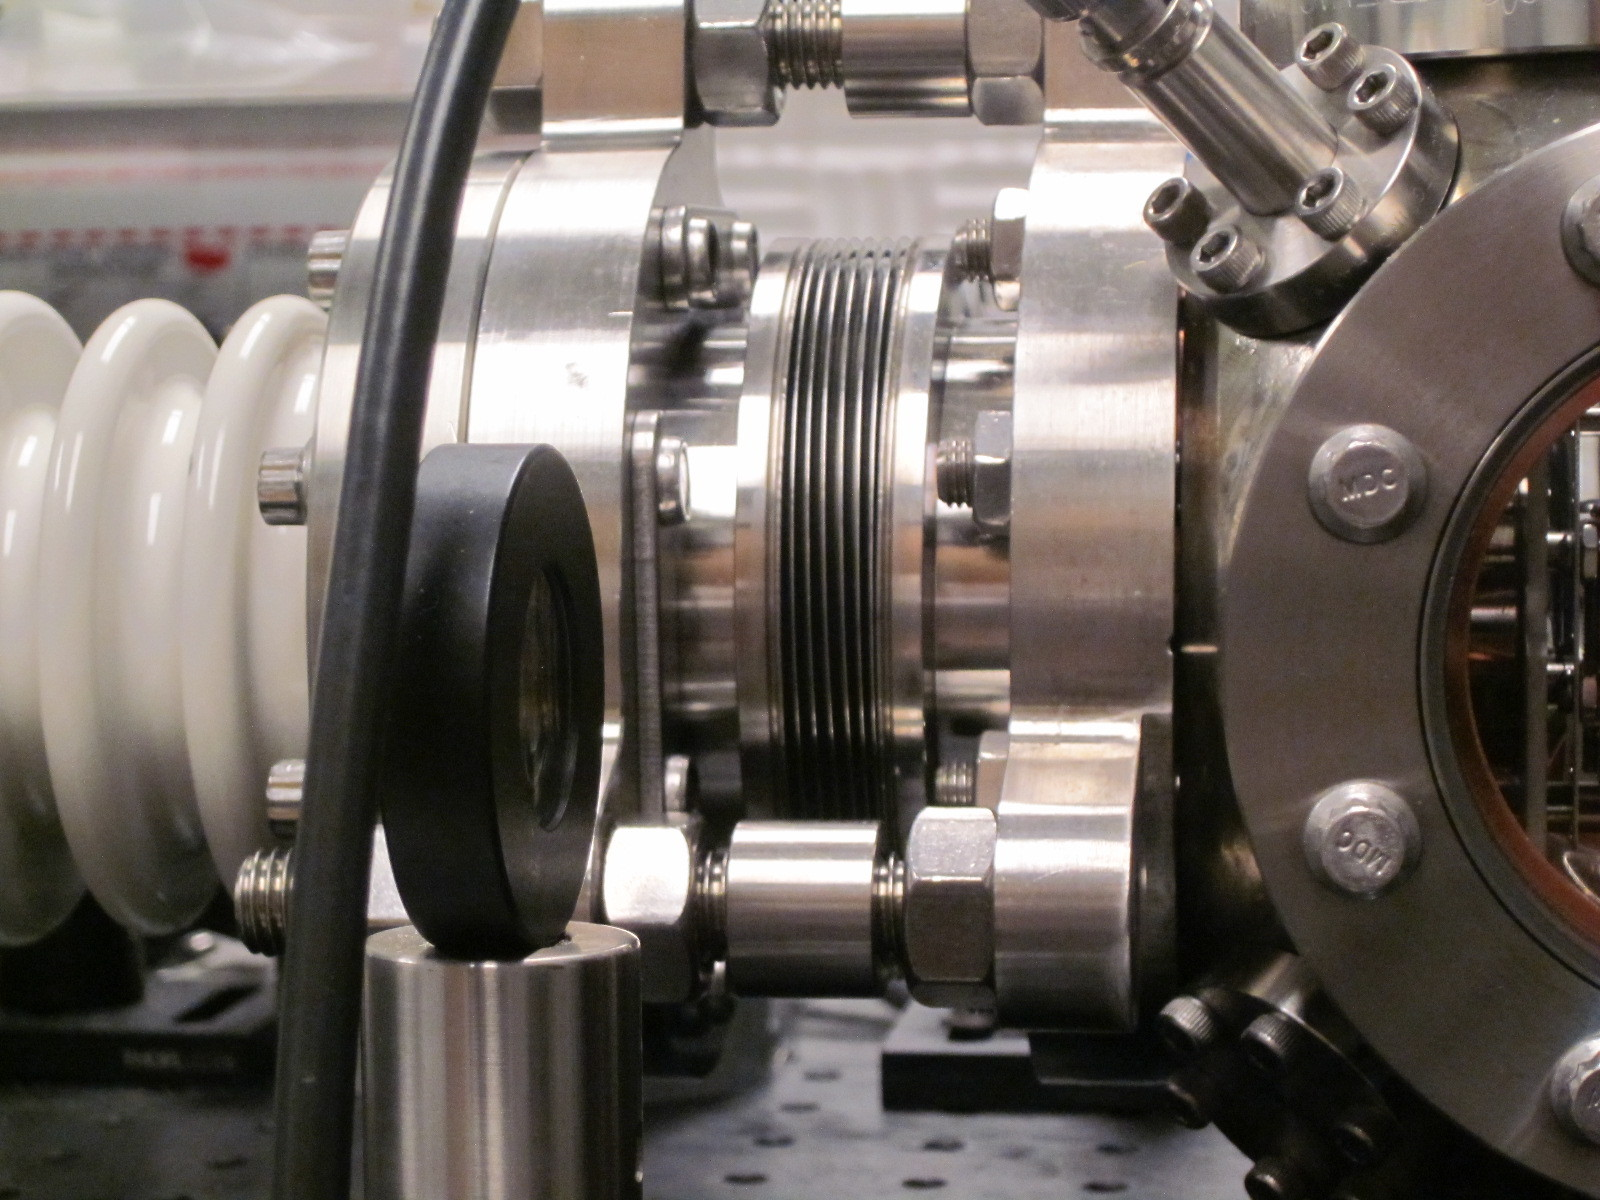
\includegraphics{aligner.jpg}
  \caption[Picture of the high-voltage side of the prototype UEM]{
    The high voltage passthrough (left) is mounted on the main chamber (right) by a ``port aligner'' which has been modified to allow coarse alignment of the cathode (mounted to the high voltage) and anode (mounted in the chamber).
  }
  \label{fig:aligner-pic}
\end{figure}



